\documentclass[11pt,letterpaper]{article}
\usepackage[utf8]{inputenc}
\usepackage[left=1in,right=1in,top=1in,bottom=1in]{geometry}
\usepackage{amsfonts,amsmath,dsfont}
\usepackage{graphicx}
% -----------------------------------
\usepackage{hyperref}
\hypersetup{%
  colorlinks=true,
  linkcolor=blue,
  citecolor=blue,
  urlcolor=blue,
  linkbordercolor={0 0 1}}
% -----------------------------------
\usepackage[authordate,backend=biber]{biblatex-chicago}
\addbibresource{citation.bib}
% -----------------------------------
\title{Learning the Evolution of Statistical Moments and Extreme Values from Data}
\author{Ryan Sh\`iji\'e D\`u}
\date{\today}
% -----------------------------------
% \setlength{\parindent}{0.0in}
\setlength{\parskip}{0.1in}
% -----------------------------------
\begin{document}
\newcommand{\de}{\mathrm{d}}
\newcommand{\DD}{\mathrm{D}}
\newcommand{\pe}{\partial}
\newcommand{\mcal}{\mathcal}
%\newcommand{\pdx}{\left|\frac{\partial}{\partial_x}\right|}

\newcommand{\dsp}{\displaystyle}

\newcommand{\norm}[1]{\left\Vert #1 \right\Vert}
%\newcommand{\mean}[1]{\left\langle #1 \right\rangle}
\newcommand{\mean}[1]{\overline{#1}}
\newcommand{\inner}[2]{\left\langle #1,#2\right\rangle}

\newcommand{\ve}[1]{\boldsymbol{#1}}

\newcommand{\thus}{\Rightarrow \quad }
\newcommand{\fff}{\iff\quad}
\newcommand{\qdt}[1]{\quad \mbox{#1} \quad}

\renewcommand{\Re}{\mathrm{Re}}
\renewcommand{\Im}{\mathrm{Im}}
\newcommand{\E}{\mathbb{E}}
\newcommand{\lap} {\nabla^2}
\renewcommand{\div}{\nabla\cdot}

\newcommand{\hot}{\text{h.o.t.}}

\newcommand{\ssp}{\left.\qquad\right.}

\newcommand{\var}{\text{var}}
\newcommand{\cov}{\text{cov}}

\newcommand{\csch}{\text{csch}}
\newcommand{\sech}{\text{sech}}

\newcommand{\MATLAB}{\textsc{Matlab}}




% -----------------------------------
\maketitle

\section{Introduction}
Assuming that the time-series data $x$ follow random variables at each time, we are often interested in the evolution of the shape of the conditional probability distribution $p(x|t)$. Learning the evolution of statistical moments is a useful proxy. Extreme values of a heavy tail random variable often correspond to significant real-world events and their changes are also worth learning from data. In this note, we propose a simple modification from linear regression that could learn the evolution of statistical moments and extreme values from data. We will explore the benefits and shortcomings of this method, and compare this method with existing methods in the literature.

\section{Linear regression for learning changes in arbitrary expectations}
Suppose in a time period $t\in [0,T]$ there is a random variable $X_t\in\mathbb{R}\times[0,T]$ that evolves in time. It has the probability density function $p(x,t)$. The expected value of $f(X_t)$ conditioned on $t$ is:
\begin{align}
    g(t) = \mathbb{E}_t[f(X_t)] = \int_\mathbb{R} f(x)p(x|t)\;\de x.\label{eq:expectation_fg}
\end{align}
We have $X_i$: samples of $X_t$ at time $t = t_i$. In this note, we will show that we can extract information about the time-change of $g(t)$ from applying least-squares fit to $f(X_i)$. Specifically, by choosing specific $f$ functions, we could diagnose the evolution of statistical moments and extreme events. For example, $f(x) = x$ gives the mean $\overline{x}(t)$ and $f(x) = (x-\overline{x}(t))^2$ gives the variance $k_2(t)$ (second cumulant) as a function of time. 

Consider the function $g(t)\in L^2([0,T])$ and a number of linearly independent basis functions $e_j(t)\in L^2([0,T])$. Linear regression finds $\sum_j\alpha_j e_j(t)$, an approximation of $g(t)$, by minimizing
\begin{align}
    \inf_{\alpha_j} \int_0^T \left[ g(t)-\sum_j\alpha_je_j(t) \right]^2\de t.
\end{align}
Since the optimization is convex, it is equivalent to setting the derivative to zero:
\begin{align}
    \int_0^T \left[ g(t)-\sum_j\alpha_je_j(t) \right]e_i(t)\;\de t = 0\label{eq:leastsq_proj}\qdt{} \text{for all $i$.}
\end{align}
We can interpret this formulation as the requirement that the residual of the fit is orthogonal to the span of the basis functions $e_j(t)$. 

Now we combine \eqref{eq:expectation_fg} and \eqref{eq:leastsq_proj} and have that if we were to apply linear regression to approximate probability expectation of $f(X_t)$ (i.e.: $\mathbb{E}[f(X_t)]$), we need to satisfy 
\begin{align}
    \int_0^T\int_\mathbb{R} \left[f(x)-\sum_j\alpha_je_j(t)\right]e_i(t)p(x,t)\;\de x\de t = 0\qdt{} \text{for all $i$}\label{eq:excp_zero}
\end{align}
where we used $\dsp{\int_\mathbb{R} p(x,t)\;\de x = 1}$ for all $t$ and $e_i(t)$'s are independent of $x$. This is equivalent to the minimization problem
\begin{align}
    \inf_{\alpha_j}\int_0^T \int_\mathbb{R} \left[f(x)-\sum_j\alpha_je_j(t)\right]^2p(x,t)\;\de x\de t.
\end{align}
Therefore to fit the time-change of $\mathbb{E}[f(X_t)] = g(t)$, we could apply the method of least-squares to the data $f(X_i)$. 

To make this explicit, as long as the data is sampled uniformly in time\footnote{If the data is not uniformly sampled in time, we should consider appropriately weighting the sum (see \cite{Du_23}).}, the double integral could be approximated as a sum. In principle, we use Monte-Carlo to approximate the probability integral and Riemann sum for the time integral. We have the minimization problem
\begin{align}
    \inf_{\ve \alpha} \left[f(X_i)-\ve A\ve \alpha\right]^T\left[f(X_i)-\ve A\ve \alpha\right]
\end{align}
where $f(X_i)$ is the vector of $f$ evaluated at $X_i$, $\ve A$ is the Vandermonde matrix with the $j$\textsuperscript{th} columns as $e_j(t_i)$, and $\ve \alpha$ is the vector with entries $\alpha_j$. Taking the gradient of the above minimization problem with respect to $\ve\alpha$, we get the discrete version of \eqref{eq:excp_zero}
\begin{align}
    \ve A^T\ve A\ve \alpha = \ve A^T f(X_i).
\end{align}
This is equivalent to the over-determined linear algebra problem
\begin{align}
    \ve A\ve \alpha = f(X_i).
\end{align}
We are in the familiar territory of linear regression.

\section{Some numerical tests for statistical moments and extreme values}\label{sec:numerical}
We apply this method to synthetic data with known probability distributions for all time and learn the trend in moments and extreme values. But the method is very general, we could choose any function $f$ and any set of basis functions $e_j$'s. 

\subsection{Learn the linear trend of statistical moments}\label{sec:numerical_mom}
In $t\in [-1,1]$, we use the Pearson system of random numbers to generate samples $X_i$ of size $50\times 365$ (50 years of daily data, see Figure \ref{fig:linMon_data}). We prescribe the four statistical moments --- mean, variance, skewness, and kurtosis --- to change linearly (black lines in Figure \ref{fig:linMom_mom} and \ref{fig:linMom_mom2}). We then apply the described method to these data, using the basis functions $e_1(t) = 1$, $e_2(t) = t$. For the four moments, we use 
\begin{align}
    &f_1(x) = x, &f_2(x) = (x-\overline{x})^2,\\
    &f_3(x) = \frac{(x-\overline{x})^3}{\kappa_2^{3/2}} & f_4(x) = \frac{(x-\overline{x})^4}{\kappa_2^{2}}
\end{align}
where $\overline{x}$ is the fitted mean, and $\kappa_2$ is the fitted variance. Note that the higher moments depend on the fitted first two moments, therefore to have good fits for the higher moments, it is important to learn the mean and variance well. However, this is not a necessary feature of our method. Different choices of $f$ could avoid this issue. For example in the next section, we will show an $f$ that does not depend on any fitted quantity. 
\begin{figure}
    \centering
    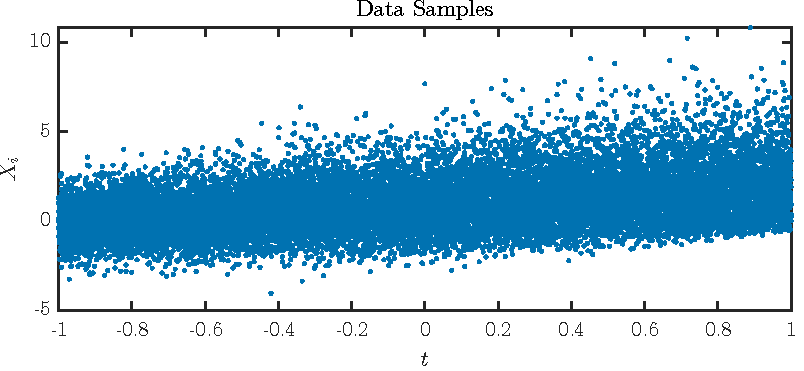
\includegraphics{figs/linMom_data}
    \caption{Synthetic data generated using the Pearson system. The four moments change linearly, they follow the black lines in Figure \ref{fig:linMom_mom}.}
    \label{fig:linMon_data}
\end{figure}

Figure \ref{fig:linMom_mom} shows a set of results of our method. We see that the learned changes match the true evolution very well. 
\begin{figure}
    \centering
    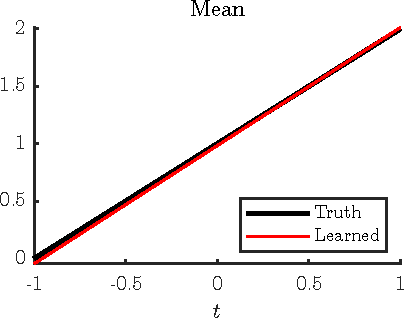
\includegraphics[width = 0.24\textwidth]{figs/linMom_mean}
    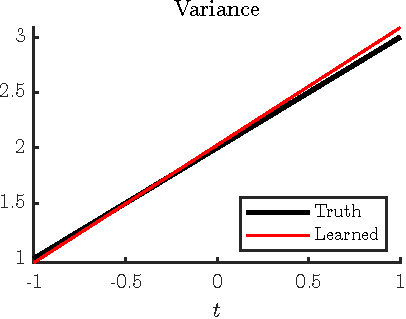
\includegraphics[width = 0.24\textwidth]{figs/linMom_var}
    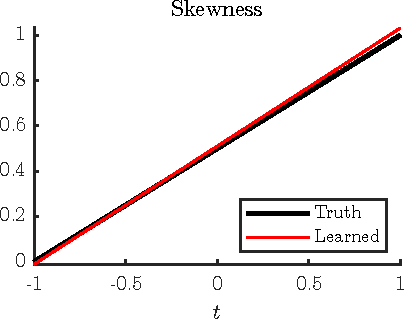
\includegraphics[width = 0.24\textwidth]{figs/linMom_skew}
    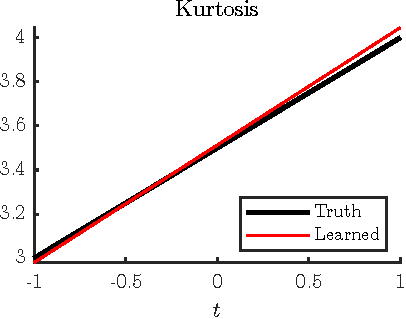
\includegraphics[width = 0.24\textwidth]{figs/linMom_kurt}
    \caption{The true evolution (black lines) and learned evolution from data (red lines) for the four moments of interest.}
    \label{fig:linMom_mom}
\end{figure}
Figure \ref{fig:linMom_mom2} shows a set where the results do not look as perfect. This is because the magnitudes of changes for the higher statistical moments are an order of magnitude less than the change in the mean. Therefore the error in the fit for the mean is relatively more influential for the fits for the higher statistical moments. From this example we see that it might not be a great practice to choose $f$ that depends on other fitted quantities.
\begin{figure}
    \centering
    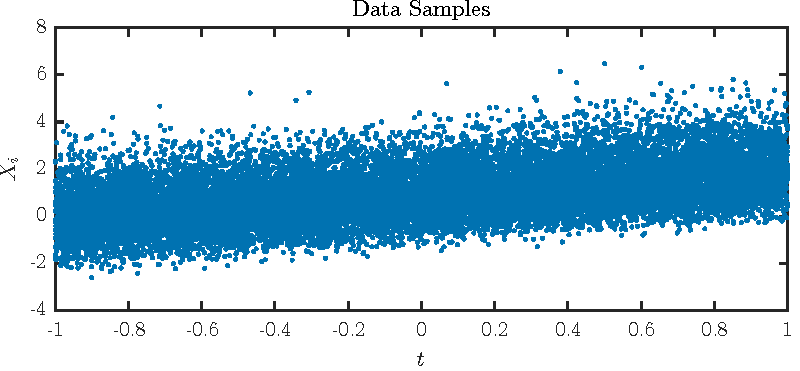
\includegraphics{figs/linMom_data2}
    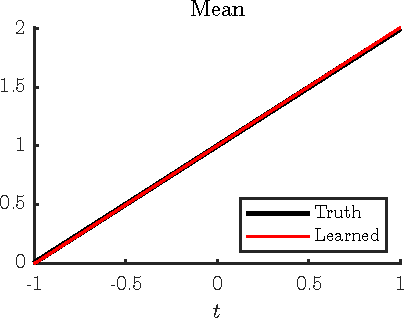
\includegraphics[width = 0.24\textwidth]{figs/linMom_mean2}
    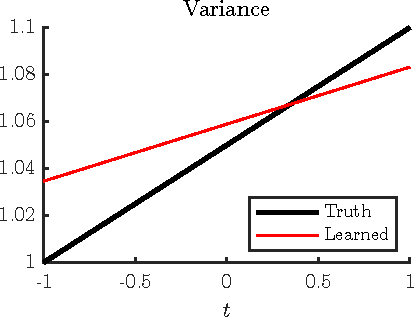
\includegraphics[width = 0.24\textwidth]{figs/linMom_var2}
    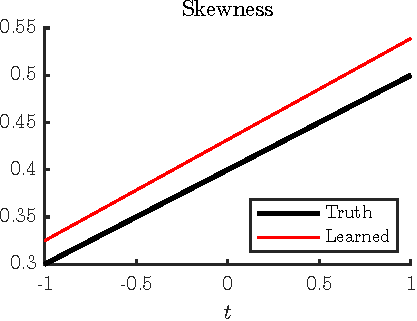
\includegraphics[width = 0.24\textwidth]{figs/linMom_skew2}
    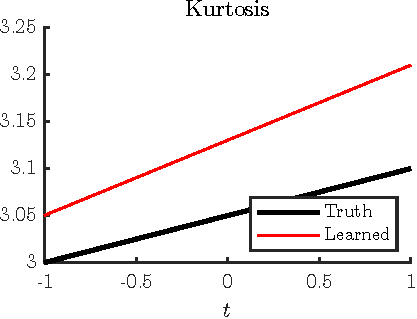
\includegraphics[width = 0.24\textwidth]{figs/linMom_kurt2}
    \caption{The top and bottom figures are similar to Figure \ref{fig:linMon_data} and \ref{fig:linMom_mom} respectively.}
    \label{fig:linMom_mom2}
\end{figure}

We comment that it is simple to apply some kind of significant testing (e.g.: the bootstrapping procedure described in \cite{FalascaEtAl_22}) to check whether there are statistically significant changes in the moments (i.e. non-zero slope). Preliminary results (not shown) indicated that it works well.

\subsection{Learn the time-change in extreme values}\label{sec:numerical_extreme}
An interesting choice for $f(x)$ is a step function $f(x) = \chi_{x > a}$. We have
\begin{align}
    \int_\mathbb{R} \chi_{x > a}p(x|t)\;\de x = \mathbb{P}(X_t>a),
\end{align}
We are learning the time change in the probability of extreme values. For example, this could be the probability of dangerously high wet-bulb temperatures, or the probability of high sea levels in a city.

We use the same data from the last section as examples. Since we are using the Pearson system of distributions, we know the true $\mathbb{P}(X_t>a)$ theoretically. We pick the threshold of $a = 5$. Because the probability of extremes changes non-linearly in time, we use $e_1(t) = 1, e_2(t) = t$, and the exponential ($e_3(t) = e^t$) as basis functions. It is conceivable that we could obtain a better fit if we choose better basis functions, informed by the mathematical theory of extremes. We show the result using the data in Figure \ref{fig:linMon_data} on the left of Figure \ref{fig:linMom_extreme}, and the result using the data in Figure \ref{fig:linMom_mom2} on the right. The method learns the change in extremely well. In particular, the result is not dependent on the fit of some other quantities. 
\begin{figure}
    \centering
    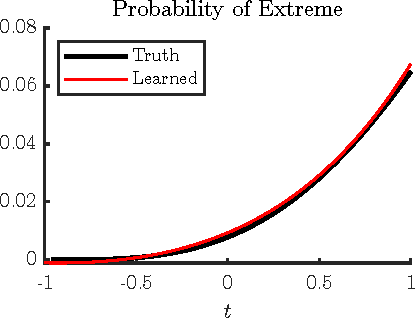
\includegraphics{figs/linMom_extreme}\hspace{10mm}
    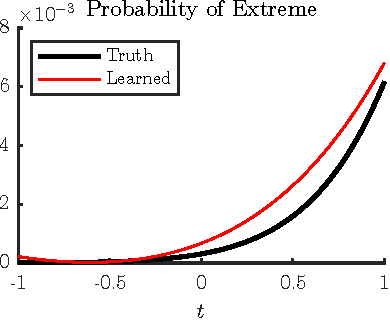
\includegraphics{figs/linMom_extreme2}
    \caption{Left: the true and fitted (learned) time-change in the probability of extremes in the data in Figure \ref{fig:linMon_data}. Right: the same for the data in Figure \ref{fig:linMom_mom2}.}
    \label{fig:linMom_extreme}
\end{figure}

We remark that $f(x)$ as a step function gives the probability of extreme values. Another choice of $f(x)$ can also account for the severity of the extremes as well. One example is the ReLU function. 

\section{Comments on the method, and comparison with existing methods}
\subsection{Benefits and deficiencies}
The method presented in this note is a simple extension of linear regression. It is easy to understand and implement for a wide array of applications. This is its main strength. The method can be improved from its current form by incorporating improvements for nonparametric regression. For example, one could choose better basis functions for a more general class of functions \parencite{Tibshirani_18}, or incorporate regularization by using a Bayesian framework \parencite{Bishop_06}. In fact, \cite{Tibshirani_18} mentioned our method for variance estimation in \S8. 

However, the method suffers from similar problems as regression. In particular, the convergence rate of the fit degrades with high-dimensional data. There are many ideas to improve the convergence behavior in the literature on high-dimensional regression that we can incorporate into our method. For example, when the parameters can be assumed to be ``sparse'', we could use LASSO \parencite{Bishop_06}.

To use our method to diagnose the change in the probability of the extreme, we need enough samples in the extreme regime so that the Monte Carlo approximation of the integral is accurate. This might not be the case for the given data set when extreme events are very rare. For these situations, one could resort to sampling techniques that are geared towards sampling the probability tails (e.g.: important sampling).

\subsection{Compare with methods in the literature}
There are many methods to diagnose variance from data, and many are discipline specific. Here we will compare our method to a few that we have seen. The list is by no means extensive.

Our method is superior to methods that bin the data to estimate statistical quantities first. For example, \cite{TankKonnen_03} listed many quantities of practical interests in climate science in form of days per year. Calculating statistical quantities in a chosen time period is equivalent to performing the Monte Carlo approximation to the probability integral in our formula per bin. Linear regression on the data calculated from each bin is an approximation of the time integral. Our calculation shows that we can combine the two steps and approximate the double integral together. This makes use of the available data efficiently. We can use our method as long as the quantity of interests can be written as a function $f(x)$ on the data.

\cite{McKinnonEtAl_16} proposed a method of calculating linear changes in quantities close to statistical moments via quantile regression. Their method was improved by \cite{FalascaEtAl_22}. Their method shows an interesting connection between linear changes in qualities to linear changes in moments-like quantities (both papers explicitly warned against interpreting their results as actual changes in moments, but called those changes as changes in mean, variance, skewness, and kurtosis). However, if one wants to diagnose the changes in moments directly, our method is numerically cheaper and more versatile. Our method can learn the nonlinear evolution of many statistical quantities not just moments, and it can be extended to higher dimensions. 

\cite{TabakTrigila_18} proposed a general framework that could be applied to our problem of moments estimation. They solved the problem of conditional density estimation (and sampling) using optimal transport in \S6. For time-series data, their method would map the data $X_t$ to $Y = Y(X_t;t)$, which follows a single random variable (the weighted barycenter) $\mu(y)$ that is independent of $t$. The map would minimize some cost measuring the introduced distortion. We can estimate or sample the conditional probability $\rho(x|t)$ by estimating or sampling $\mu(y)$ and using the inverse maps. Estimating moments is then an easy extension. Although the adaptation of their framework to estimate higher moments is not trivial, we believe that it has promise to outperform our method in high-dimension, data-poor regimes. Additionally, its unifying approach connects many common methods in an intellectually satisfying way and extends them. Anyone who is interested in estimating the evolution of probability distribution over parameters should consider their methods. However, we think our method is useful in its simplicity. It works well as a quick tool for proof of concepts.

\section*{Acknowledgment}
This note was inspired by a talk by Andrew Brettin. We thank him and Fabrizio Falasca for explaining the methods in \cite{McKinnonEtAl_16} and \cite{FalascaEtAl_22}. Many conversations with experts have improved this note. We thank Jonathan Niles-Weed for situating our work in the field of nonparametric estimation and pointing us to \cite{Tibshirani_18}. We thank Esteban Tabak for introducing us to \cite{TabakTrigila_18}. 

\newpage
\printbibliography

\end{document}
